\documentclass[sigconf,review,anonymous]{acmart}

\usepackage{booktabs} % For formal tables

% Copyright
\setcopyright{none}
%\setcopyright{acmcopyright}
%\setcopyright{acmlicensed}
%\setcopyright{rightsretained}
%\setcopyright{usgov}
%\setcopyright{usgovmixed}
%\setcopyright{cagov}
%\setcopyright{cagovmixed}


% DOI
\acmDOI{10.475/123_4}

% ISBN
\acmISBN{123-4567-24-567/17/06}

%Conference
\acmConference[SIGGRAPH 2017 Talks]{SIGGRAPH 2017 Talks}{August 2017}{Los Angeles, CA, USA} 
\acmYear{2017}
\copyrightyear{2017}
\acmPrice{15.00}

% use the "authoryear" citation style.
\citestyle{acmauthoryear}
\setcitestyle{square}

\begin{document}
\title{A Two-Page Abstract Using the New Article Format}

\author{Ben Trovato}
\orcid{1234-5678-9012}
\affiliation{%
  \institution{Institute for Clarity in Documentation}
  \streetaddress{P.O. Box 1212}
  \city{Dublin} 
  \state{Ohio} 
  \postcode{43017-6221}
}
\email{trovato@corporation.com}

\author{G.K.M. Tobin}
\affiliation{%
  \institution{Institute for Clarity in Documentation}
  \streetaddress{P.O. Box 1212}
  \city{Dublin} 
  \state{Ohio} 
  \postcode{43017-6221}
}
\email{webmaster@marysville-ohio.com}

% The default list of authors is too long for headers}
\renewcommand{\shortauthors}{B. Trovato et. al.}

\begin{teaserfigure}
  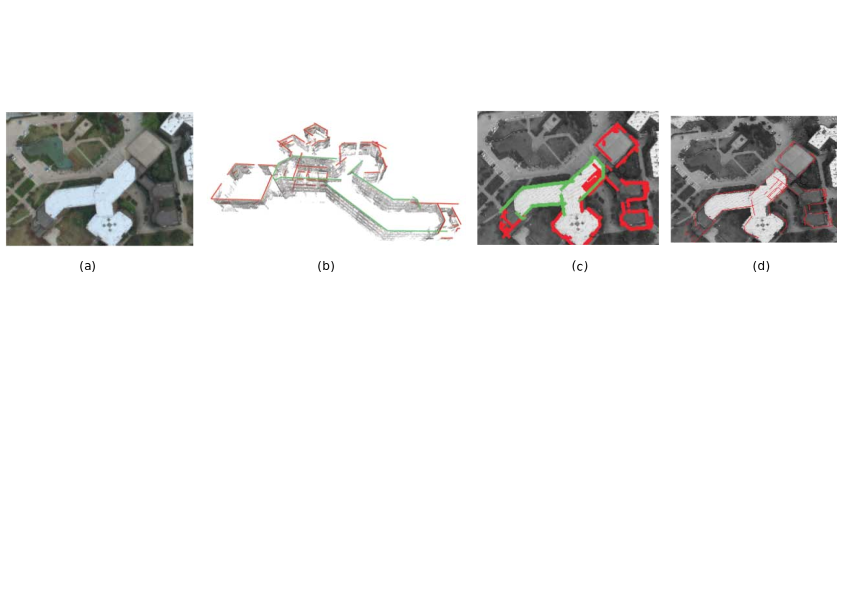
\includegraphics[width=\textwidth]{figures/teaser_pdf}
  \caption{This is a teaser image.}
  \label{fig:teaser}
\end{teaserfigure}


\maketitle

\section{Introduction}
%
As a key technique to image-based navigation, augmented reality (AR) and 3D reconstruction, geo-localization has drawn massive attentions in the literature. When presenting a geo-localization problem, an image or a frame of video is often used as the query data, a 3D model is needed to provide a global coordinate, a sensor prior is optionally employed and the camera pose with respect to the global coordinate system is to be estimated. 

In this work, we estimate the camera pose using an overhead image captured by a low-altitude aerial device as query and a corresponding building point cloud as 3D model. Comparing to existing methods using images captured on the ground~\cite{instant} or in high altitude~\cite{FDCM}, we are not able to take advantages of vanishing points and suffer from more critical perspective effect. There are two key observations that vertical facades of a point cloud correspond to edges of building roofs in the overhead image and that roofs at different altitudes are of different scales in the image, which inspires us to treat this geo-localization problem as a combination of a multi-layer shape matching problem and a global optimizing procedure. 
%利用这个方法,我们可以。。。。。
%
 \begin{figure}
 	\centering
 	\vspace{2.0cm}
 	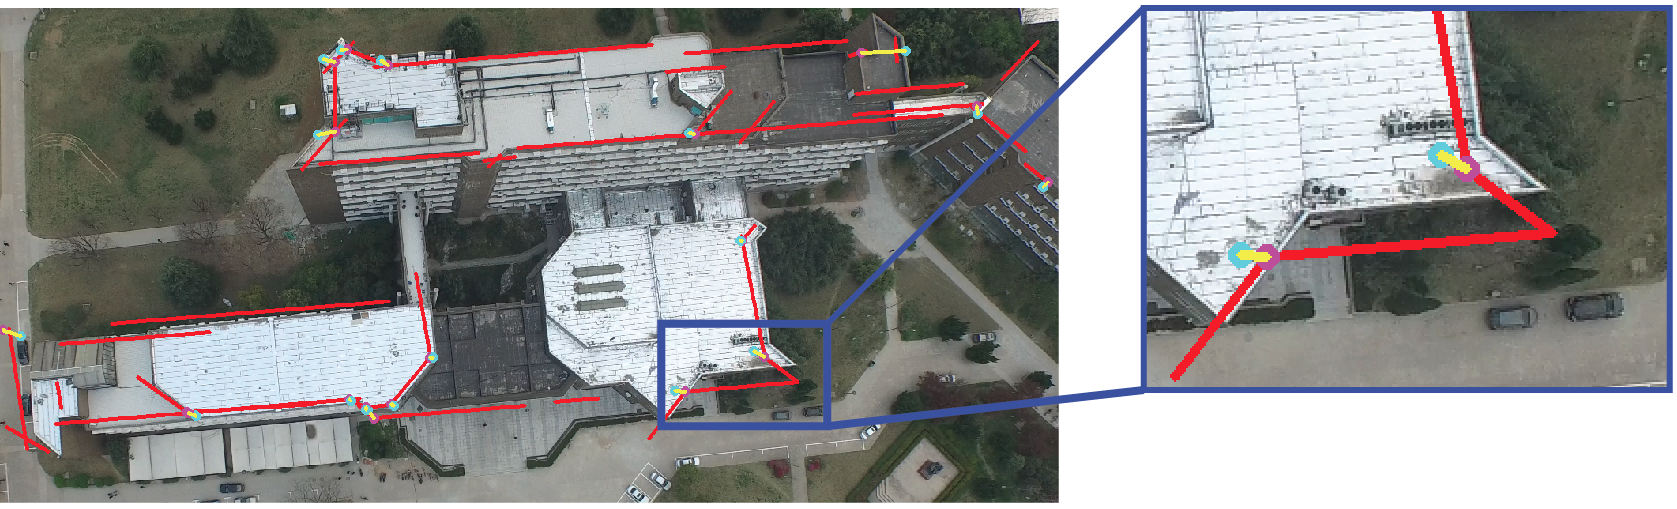
\includegraphics[width=0.5\textwidth]{figures/details_png}
 	\caption{Finding paired 3D and 2D feature points: for a 3D feature point, we project it on the overhead image (magenta points) using current project matrix and search in its $k\times k$ neighborhood for a corner (cyan points). These 3D feature points and corresponding corners will form pairs of feature points for next iteration of calculating global matrix.}
 	\label{fig:overview}
 \end{figure}
\section{Our Approach}
Given a building point cloud, we first extract contours of building roofs in different altitudes according to the altitude histogram of points, where each contour is fit into a set of line segments (Figure 1b). And then the contours are matched with the edge map of the overhead image respectively using a shape matching technique of \cite{FDCM}. A local project matrix is achieved for each contour (Figure 1c). Note that we need a global project matrix instead of local ones to estimate the camera pose. So we treat the result of shape matching as the initialization of the following global optimizing procedure. 

To calculate the global project matrix between the whole point cloud and the overhead image, we need a series of paired 3D feature points and corresponding 2D feature points. We use the intersections of neighboring line segments of building roof contours as 3D feature points and introduce an iterative algorithm to find corresponding 2D feature points, where we utilize the result of shape matching as initial project matrix.
%For each 3D feature point, we search the $k\times k$ neighborhood of its corresponding point in the overhead image after shape matching, and find a corner as its paired 2D feature point (Figure 2).
As shown in Figure~2, for a 3D feature point, we project it on the overhead image (magenta points) using current project matrix and search in its $k\times k$ neighborhood for a corner (cyan points). These 3D feature points and corresponding corners form pairs of feature points for next iteration of calculating project matrix.
%Once a set of paired 3D and 2D feature points is achieved, we randomly select a subset of these feature point pairs to calculate a global matrix. 
With this set of paired 3D and 2D feature points, we can optimize a global project matrix by minimizing the average of the distance between projected contours and the edge of the overhead image, which can be accelerated by distance transformation. With the global project matrix and pre-calibrated focus length of the camera, we can finally estimate the 6 DoF camera pose of the overhead image in point cloud coordinate system.
% Be more specific?

We tested the proposed approach on a newly collected dataset. Figure 1(d) shows one of the results, where we project roof contours onto the overhead image. Since most of the consuming time is spent in the shape matching stage and the optimizing stage is fast, we can easily extend our approach to video-based problem. 

\bibliographystyle{ACM-Reference-Format}
\bibliography{Alignment_of_Model} 

\end{document}
